% 二项分布
% 二项分布|两点分布

\pentry{二项式定理\upref{BiNor}}
\subsection{二项分布}
如果记$X $为$n $重伯努利试验中成功(记为事件$A$)的次数,则$X $的可能取值为$0,1,···,n$.记$p $为每次试验中$A $发生的概率,即$P(A)=p$,则$P(\overline{A})=1-p$.

而我们知道,$n$重伯努利试验的基本结果可以记作
\begin{equation}
\omega=\left(\omega_{1}, \omega_{2}, \cdots, \omega_{n}\right)
\end{equation}
其中$\omega_i$为$A$,或者为$\overline{A}$.这样的$\omega$共有$2^n$个,这$2^n$个样本点$\omega$组成了样本空间$\Omega$.

下面求事件$X$的分布列,即$\{X=k\}$的概率.若某个样本点
\begin{equation}
\omega=\left(\omega_{1}, \omega_{2}, \cdots, \omega_{n}\right) \in\{X=k\}
\end{equation}
意味着$\omega_1,\omega_2,\cdots,\omega_n$中有$k$个$A$,$n-k$个$\overline A$.由事件的独立性知:
\begin{equation}
P(\omega)=p^{k}(1-p)^{n-k}
\end{equation}
而事件$\{X=k\}$中这样的$\omega$共有$\binom nk$个,所以$X$的分布列为:
\begin{equation}
P(X=k)=\binom nk p^{k}(1-p)^{n-k}, k=0,1, \cdots, n
\end{equation}
这个分布成为\textbf{二项分布},记为$X\sim b(n, p)$.

那么它的和是不是为$1$呢?这很容易验证.我们有
\begin{equation}
\sum_{k=0}^{n}\binom nk p^{k}(1-p)^{n-k}=[p+(1-p)]^{n}=1
\end{equation}
并且从上式可以看出,二项概率$\binom nk p^{k}(1-p)^{n-k}$恰好是二项式$[p+(1-p)]^{n}$的展开式中的第$k+1$项,这正是其名称的由来.

显然,二项概率是一种离散分布.它很常见,举例来说:
\begin{example}{二项分布的例子}
\begin{itemize}
\item 检查$10$件产品,$ 10 $件产品中不合格品的个数$X $服从二项分布$b(10,p)$,其中$p$为不合格品率.
\item 调查$50 $个人,$ 50 $个人中患色盲的人数$Y $服从二项分布$b(50,p)$,其中$p$为色盲率.
\item 射击$5 $次,$ 5 $次中命中次数$Z $服从二项分布$b(5,p)$,其中$p $为射手的命中率.
\end{itemize}
\end{example}

下面来计算一些具体的例题.
\begin{example}{治愈的概率}
某特效药的临床有效率为$0. 95$,今有$10 $人服用,问至少有$8 $人治愈的概率是多少?

直接计算,我们有
\begin{equation}
\begin{aligned} P(X \geqslant 8) &=P(X=8)+P(X=9)+P(X=10) \\ &=\binom{10}{8} 0.95^{8} 0.05^{2}+\binom{10}{9} 0.95^{9} 0.05+\binom{10}{10} 0.95^{10} \\ &=0.0746+0.3151+0.5988=0.9885 \end{aligned}
\end{equation}
即$10 $人中有$8 $人以上被治愈的概率为$0. 988 5$.
\end{example}

\begin{example}{}
设随机变量$X\sim b(2,p),Y\sim b(3,p)$.若$P (X\geqslant1) = 5/9$, 试求$P(Y\geqslant1)$.

由$P(X\geqslant1)=5/9$,知$P(X=0)=4/9$,所以$(1-p)^2=4/9$,由此得$p=1/3$.再由$Y\sim b(3,p)$可得
\begin{equation}
P(Y \geqslant 1)=1-P(Y=0)=1-\left(1-\frac{1}{3}\right)^{3}=\frac{19}{27}
\end{equation}
\end{example}

\subsection{二点分布}
$n=1$时的二项分布$b (1 ,p)$称为\textbf{二点分布},或称 \textbf{0-1 分布},或称\textbf{伯努利分布}.其分布列为
\begin{equation}
P(X=x)=p^{x}(1-p)^{1-x}, x=0,1
\end{equation}
或者,用表格可以列为:
\begin{equation}
\begin{array}{|c|c|c|}\hline x & 0 & 1 \\ \hline P & 1-p & p \\ \hline  \end{array}
\end{equation}

二点分布$b(1 ,p) $主要用来描述一次伯努利试验中成功(记为$A$)的次数($0$或$1$).很多随机现象的样本空间$\Omega$常可一分为二,记为$A $与$\overline A$,由此形成伯努利试验.$n $重伯努利试验是由$n $个相同的、独立进行的伯努利试验组成,若将第$i $个伯努利试验中$A $出现的次数记为$X_i (i= 1,2, \cdots, n)$, 则$X_i$相互独立,且服从相同的二点分布$b(1 ,p)$.此时其和$X=X_1+X_2+\cdots+X_n$就是$n $重伯努利试验中$A $出现的总次数,它服从二项分布$b(n,p)$.这就是二项分布$b (n ,p) $与二点分布$b(1,p)$之间的联系,即服从二项分布的随机变量是$n$个独立同为二点分布的随机变量之和.

\subsection{二项分布的数学期望和方差}

设随机变量$X\sim b(n,p)$,则
\begin{equation}
\begin{aligned} E(X) &=\sum_{k=0}^{n} k\binom{n}{k} p^{k}(1-p)^{n-k}=n p \sum_{k=1}^{n}\binom{n-1}{k-1} p^{k-1}(1-p)^{(n-1)} \\ &=n p[p+(1-p)]^{n-1}=n p \end{aligned}
\end{equation}
又因为
\begin{equation}
\begin{aligned} E\left(X^{2}\right) &=\sum_{k=0}^{n} k^{2}\binom{n}{k} p^{k}(1-p)^{n-k}=\sum_{k=1}^{n}(k-1+1) k\binom{n}{k} p^{k}(1-p)^{n-k} \\ &=\sum_{k=1}^{n} k(k-1)\binom{n}{k} p^{k}(1-p)^{n-k}+\sum_{k=1}^{n} k\binom{n}{k} p^{k}(1-p)^{n-k} \\ &=\sum_{k=2}^{n} k(k-1)\binom{n}{k} p^{k}(1-p)^{n-k}+n p \\ &=n(n-1) p^{2} \sum_{k=2}^{n}\binom{n-2}{k-2} p^{k-2}(1-p)^{(n-2)-(k-2)}+n p \\ &=n(n-1) p^{2}+n p \end{aligned}
\end{equation}

由此得$X $的方差为
\begin{equation}
\operatorname{Var}(X)=E\left(X^{2}\right)-(E(X))^{2}=n(n-1) p^{2}+n p-(n p)^{2}=n p(1-p)
\end{equation}
因为二点分布是$n=1$时的二项分布$b(1,p)$,所以二点分布的数学期望为$p$,方差为$p(1-p)$.

为了看出不同的$p $的值,其二项分布$b(n ,p) $的变化情况,我们给出$n=10$时,不同$p $值的二项分布的概率值:
\begin{table}[ht]
\centering
\caption{二项分布 $b(n, p)$}\label{BiDist_tab1}
\begin{tabular}{|c|c|c|c|c|c|c|c|c|c|c|c|}
\hline
k & 0 & 1 & 2 & 3 & 4 & 5 & 6 & 7 & 8 & 9 & 10 \\
\hline
b(10,0.2) & 0.107 & 0.268 & 0.302 & 0.201 & 0.088 & 0.027 & 0.006 & 0.001 & & & \\
\hline
b(10,0.5) & 0.001 & 0.010 & 0.044 & 0.117 & 0.205 & 0.246 & 0.205 & 0.117 & 0.044 & 0.010 & 0.001 \\
\hline
b(10,0.8) & & & & 0.001 & 0.006 & 0.027 & 0.088 & 0.201 & 0.302 & 0.268 & 0.107 \\
\hline
\end{tabular}
\end{table}
我们再来看一下按照上面的数据描绘出的线条图:
\begin{figure}[ht]
\centering
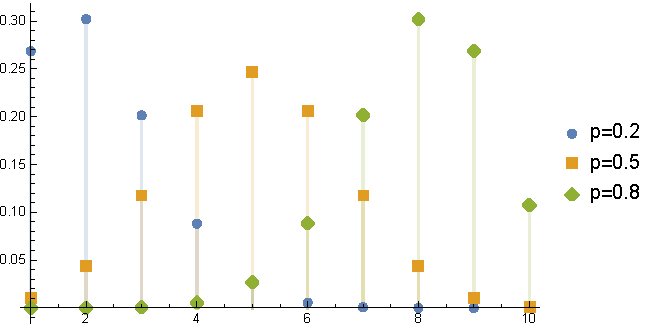
\includegraphics[width=10cm]{./figures/BiDist_1.pdf}
\caption{二项分布$b(n,p)$的线条图} \label{BiDist_fig1}
\end{figure}

从上图可以看出:
\begin{itemize}
\item 位于均值$np$附近概率较大.
\item 随着$p $的增加,分布的峰逐渐右移.
\end{itemize}

下面来看一个例题.
\begin{example}{}
甲、乙两棋手约定进行$10 $局比赛,以赢的局数多者为胜.设在每局中甲赢的概率为$0.6$,乙赢的概率为$0. 4$.如果各局比赛是独立进行的,试问甲胜、乙胜、不分胜负的概率各为多少?

以$X $表示$10 $局比赛中甲赢的局数,则$X\sim b(10,0. 6)$.所以
\begin{equation}
\begin{aligned}P(\text { 甲胜 })=P(X \geqslant 6)=\sum_{k=6}^{10}\binom{10}{k} 0.6^{k} 0.4^{10-k}=0.6330 \\ P(\text { 乙胜 })=P(X \leqslant 4)=\sum_{k=0}^{4}\binom{10}{k} 0.6^{k} 0.4^{10-k}=0.1663 \\ P(\text { 不分胜负 })=P(X=5)=\binom{10}{5} 0.6^{5} 0.4^{5}=0.2007\end{aligned}
\end{equation}
可见甲胜的可能性达$63. 3\%$,而乙胜的可能性只有$16. 63\% $,它比不分胜负的可能性还要小.最后两个概率之和$0. 367 0 $表示乙不输的概率.
\end{example}